\section{Arbeitsgrundlagen}

\begin{figure}[H]
    \centering
    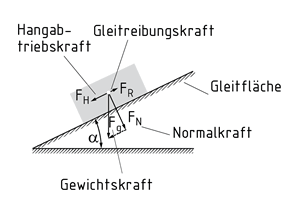
\includegraphics[width=.7\linewidth]{images/gleitreibung_hang}
    \caption{Die Verschiedenen Kr\"afte, die auf ein Objekt Wirkung haben.}
    \label{fig:objekt}
\end{figure}

Ein       Objekt       mit       der       Masse       $m$        wird       mit
$g\approx\SI{9.81}{\meter\per\second\squared}$  gegen   Erde  beschleunigt.  Die
\textit{Gewichtskraft} $F_g$ ist somit:

\begin{equation}
    F_g = m \cdot g
\end{equation}

Falls das Objekt sich  auf  einer  ungeraden Ebene befindet mit winkel $\alpha$,
wird  die Gewichtskraft $F_g$ in zwei auf sich senkrechte  Vektoren  aufgeteilt:
Die \textit{Normalkraft} $F_N$ und  die  \textit{Hanabtriebskraft}  $F_H$ (siehe
auch  Abbildung \ref{fig:objekt}). Je nach Winkel $\alpha$ wird die  Normalkraft
st\"arker oder Schw\"acher.

\begin{align}
    F_N &= F_G\cdot\cos\alpha \\
    F_H &= F_G\cdot\sin\alpha
\end{align}

Je nach Material des  Objekts  und  Material der Fl\"ache entseht eine bremsende
Kraft,   die   sogenannte   \textit{Reibungskraft}   $F_R$,   welche   in    die
entegengesetzte Richtung der Hangabtriebskraft $F_H$ wirkt.  Ist $F_R$ gr\"osser
als $F_H$, dann bleibt  das  Objekt  stehen.  Ist  sie kleiner, dann rutscht das
Objekt mit zunehmender Geschwindigkeit die Fl\"ache hinunter.

Die Reibungskraft wird  unterteilt  in eine \textit{Grenthaftkraft} $F_{H0}$ und
eine  \textit{Gleitreibungskraft} $F_{gl}$. Wenn  das  Objekt  stillsteht,  dann
wirkt eine Reibungskraft, der  genau  gleich gross ist wie die Hangabtriebskraft
$F_H$, die das Objekt stillh\"alt. Diese Kraft wirkt solange, bis sie  gr\"osser
wird als die Grenzhaftkraft $F_{H0}$. Danach beginnt das Objekt zu rutschen, und
es wirkt die Gleitreibungskraft $F_{gl}$.

In der Abbildung \ref{fig:haft_gleit_uebergang} ist dieser Vorgang visualisiert.

\begin{figure}[H]
    \centering
    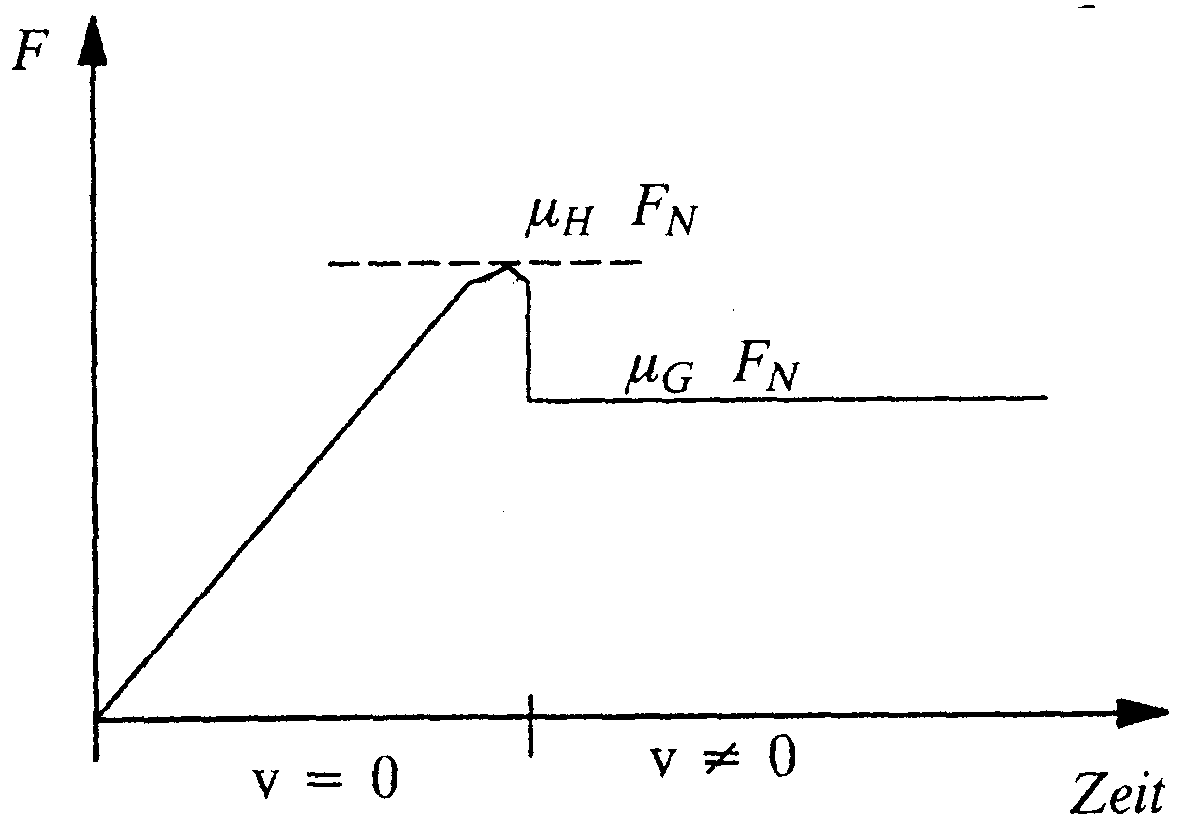
\includegraphics[width=.7\linewidth]{images/haft_gleit_uebergang}
    \caption{\"Ubergang eines stillstehenden Objektes zu einem rutschenden Objekt.}
    \label{fig:haft_gleit_uebergang}
\end{figure}

Die beiden Reibungskr\"afte k\"onnen mit den folgenden Formeln berechnet werden.

\begin{align}
    F_{H0} = \micro_H\cdot F_N \\
    F_{gl} = \micro_G\cdot F_N
\end{align}

Wobei  $\micro_H$   und   $\micro_G$   materialabh\"angig  sind.  Weiter  ist
interessant  zu beachten, dass die Reibungskr\"afte geschwindigkeitsunabh\"angig
sind. Nat\"urlich wird $F_{H0}$ immer gr\"osser sein als $F_{gl}$.

